\documentclass[11pt]{article}

\usepackage{graphicx}
\usepackage{amsmath,amsfonts,amssymb}

\usepackage{hyperref}  % for urls and hyperlinks
\setlength{\textwidth}{6.2in}
\setlength{\oddsidemargin}{0.3in}
\setlength{\evensidemargin}{0in}
\setlength{\textheight}{8.9in}
\setlength{\voffset}{-1in}
\setlength{\headsep}{26pt}
\setlength{\parindent}{0pt}
\setlength{\parskip}{5pt}

% matrix environment
\newenvironment{mat}{\left[ \begin{array}{ccccccccccccc}}{\end{array}\right]}
\newcommand\bcm{\begin{mat}}
\newcommand\ecm{\end{mat}}

\begin{document}

\hfill\vbox{\hbox{AMath 574}\hbox{Homework 4}
\hbox{Jithin George}}




%--------------------------------------------------------------------------

\vskip 1cm
\hrule
\begin{enumerate} 
\item
(Adapted from Exercise 13.7 in the book)

{\bf Note:} The Jupyter notebook {\tt homeworks/hw4/Homework4-p-system.ipynb} 
will get you started on some parts of this problem (in particular parts (d),
(e) and (g) are solved already).  You can add
to this notebook to produce the other plots you need and also adapt it for
parts of Problem 2 below.

Consider the p-system (described in Section 2.13),
\begin{equation*}
\begin{split} 
v_t - u_x &= 0,\\
u_t + p(v)_x &= 0,
\end{split} 
\end{equation*}
where $p(v)$ is a given function of $v$.
Note that $q = [v,~u]^T$ for this system.
\begin{enumerate} 
\item Compute the eigenvalues of the Jacobian matrix and show that the
system is hyperbolic provided $p'(v)<0$.

\vskip 1cm
{\bf Solution:}
\begin{equation*}
\begin{split} 
v_t - u_x &= 0,\\
u_t + p'(v) v_x &= 0,
\end{split} 
\end{equation*}
So, 
\[ A= \bcm 0 & -1 \\ p'(v) & 0 \ecm \]

The eigenvalues are $\pm \sqrt{-p'(v)}$. So , for the system to be hyperbolic, $p'(v)$ has to be less than zero.

\item Use the Rankine-Hugoniot condition to show that a shock connecting
$q=(v,u)$ to some fixed state $q^*=(v^*,u^*)$ must satisfy
\begin{equation} 
u = u_* \pm \sqrt{-\left( \frac{p(v)-p(v_*)}{v-v_*} \right)} ~(v-v_*).
\end{equation}

\vskip 1cm
{\bf Solution:}

\[ s= \frac{f(q1_*)-f(q1)}{q1_*-q1}=\frac{f(q2_*)-f(q2)}{q2_*-q2}\]
\[ s= \frac{-(u_*-u)}{v_*-v}=\frac{p(v_*)-p(v)}{u_*-u}\]
\[ (u_*-u)^2=-(p(v_*)-p(v))(v_*-v)\]
\[ u_*=u \pm \sqrt{-(p(v_*)-p(v))(v_*-v)}\]
\[u_* = u \pm \sqrt{-\left( \frac{p(v)-p(v_*)}{v-v_*} \right)} ~(v-v_*)\]
\item What is the propagation speed for such a shock?  How does this relate
to the eigenvalues of the Jacobian matrix computed in part (a)?

\vskip 1cm
{\bf Solution:}
\[ s= \frac{-u_*+u}{v*-v}=\pm \sqrt{-\left( \frac{p(v)-p(v_*)}{v-v_*} \right)}\]

As v gets very close to $v_*$, the shock speeds are the same as the eigenvalues.
\item Plot the Hugoniot loci for the point $q_* = (1,1)$ over the range
$-3\leq v \leq 5$ for the case $p(v) = -e^v$.

{\bf Note:} This is not a realistic equation of state for a gas if $v$
represents the specific volume $1/\rho$ as described in Section 2.13, since
in that case $v>0$ is required and $p(v) \rightarrow \infty$ as
$v\rightarrow 0$.  But mathematically this gives a fine hyperbolic system.

\vskip 1cm
{\bf Solution:}


	\begin{minipage}{\linewidth}
		\centering
	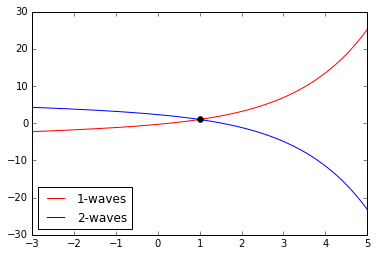
\includegraphics[width=8cm]{d.png}
	\end{minipage}

\item Determine the 2-shock solution to the Riemann problem for the p-system
with $p(v) = -e^v$ and data
\[
q_\ell = (1,1), \qquad q_r = (4,3).
\]
Do this in two ways:
 \begin{enumerate} 
 \item Plot the relevant Hugoniot loci and estimate where they intersect.
 \item Set up and solve the proper scalar nonlinear equation for $v_m$, 
 using \verb+scipy.optimize.fsolve+.
 \end{enumerate} 
\vskip 1cm
{\bf Solution:}


\begin{minipage}{\linewidth}
	\centering
	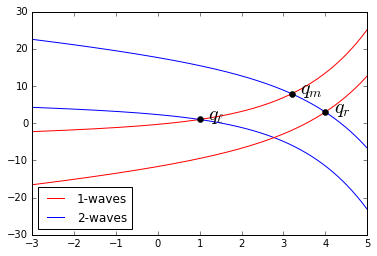
\includegraphics[width=8cm]{e.png}
\end{minipage}

Using fsolve, we get 
\[q_m = \bcm 3.19779 \\  7.91551 \ecm \]
\item Does the Riemann solution found in the previous part
satisfy the Lax Entropy
Condition?  Sketch the structure of the solution in the $x$-$t$ plane
showing also some sample 1-characteristics and 2-characteristics.

\vskip 1cm
{\bf Solution:}
\[v_l<v_m<v_r\]
\[ \lambda_1 = -e^{v/2} \]
Thus, for $\lambda_1$,
 \[ \lambda_l>\lambda_m\]
 This satisfies the condition for a 1-shock.
 However,
 for $\lambda_2  = e^{v/2}$,
 \[ \lambda_m<\lambda_r\]
 Thus, it is a 2-rarefaction. So, it does not satisfy the Lax Entropy condition. 
 \vskip 1cm
 The 1-charactersitics :
 
 \begin{minipage}{\linewidth}
 	\centering
 	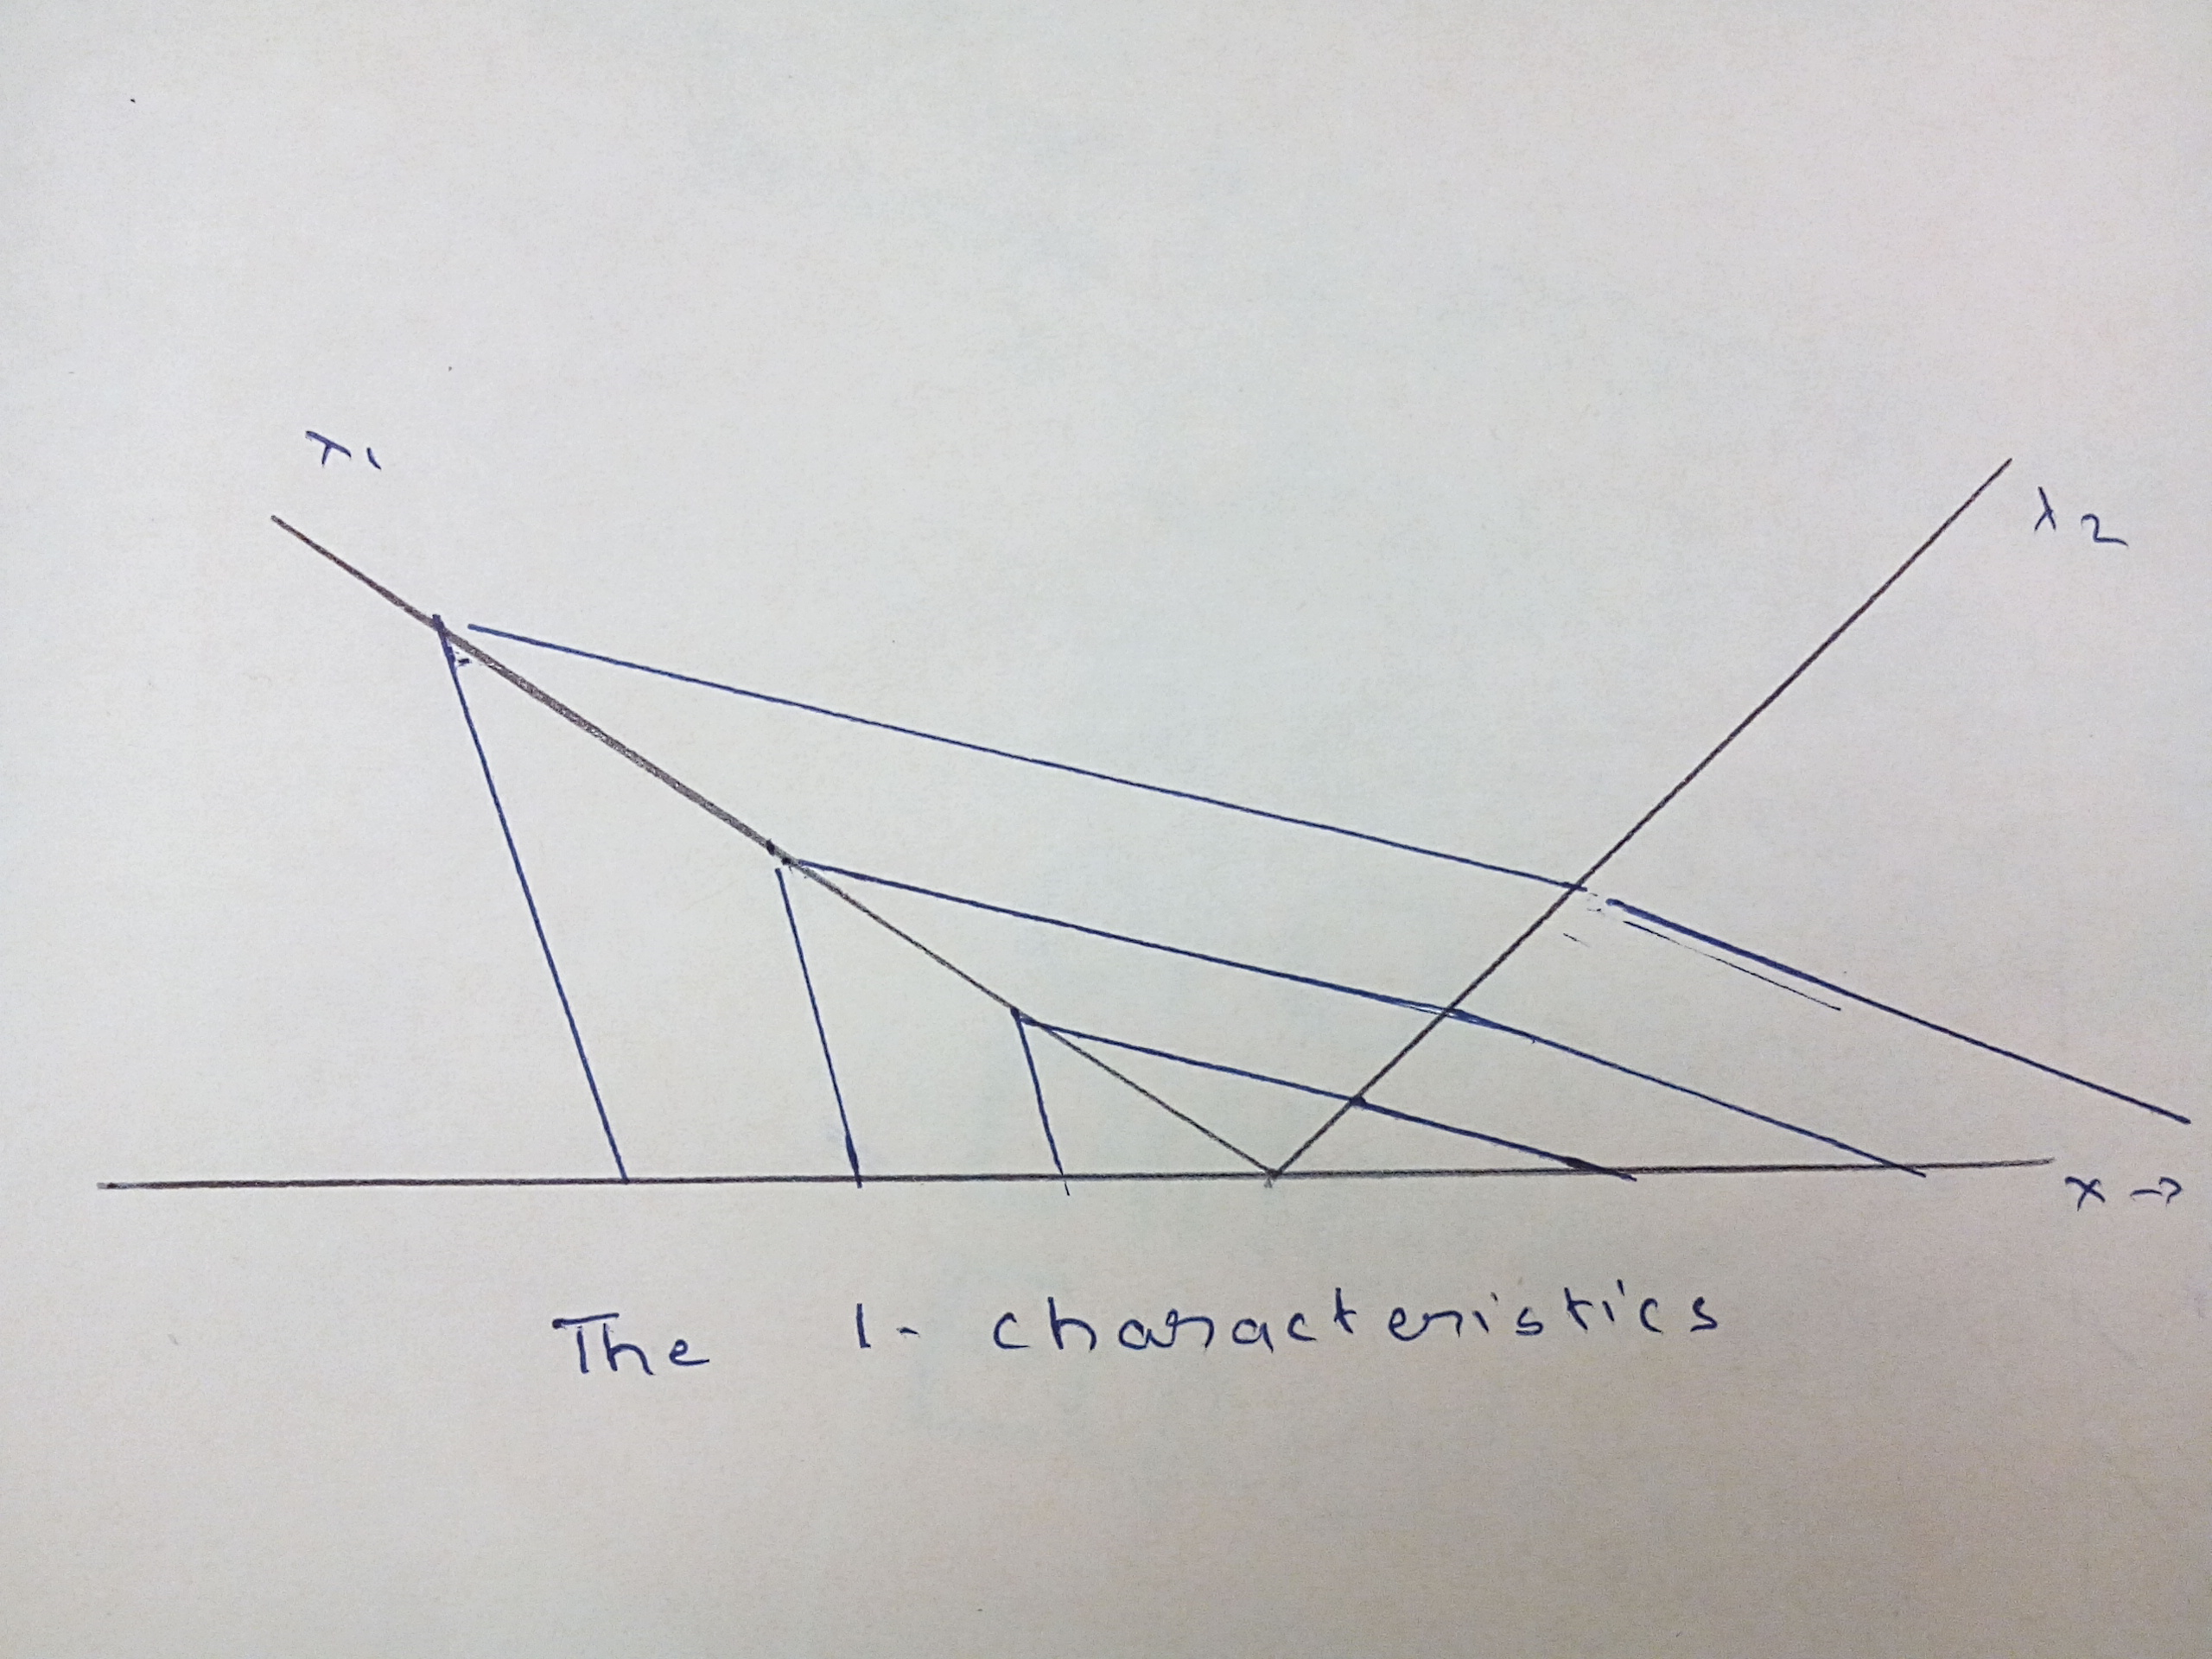
\includegraphics[width=8cm]{im1}
 \end{minipage}
 
 \vskip 1cm
  The 2-charactersitics :
  
  \begin{minipage}{\linewidth}
  	\centering
  	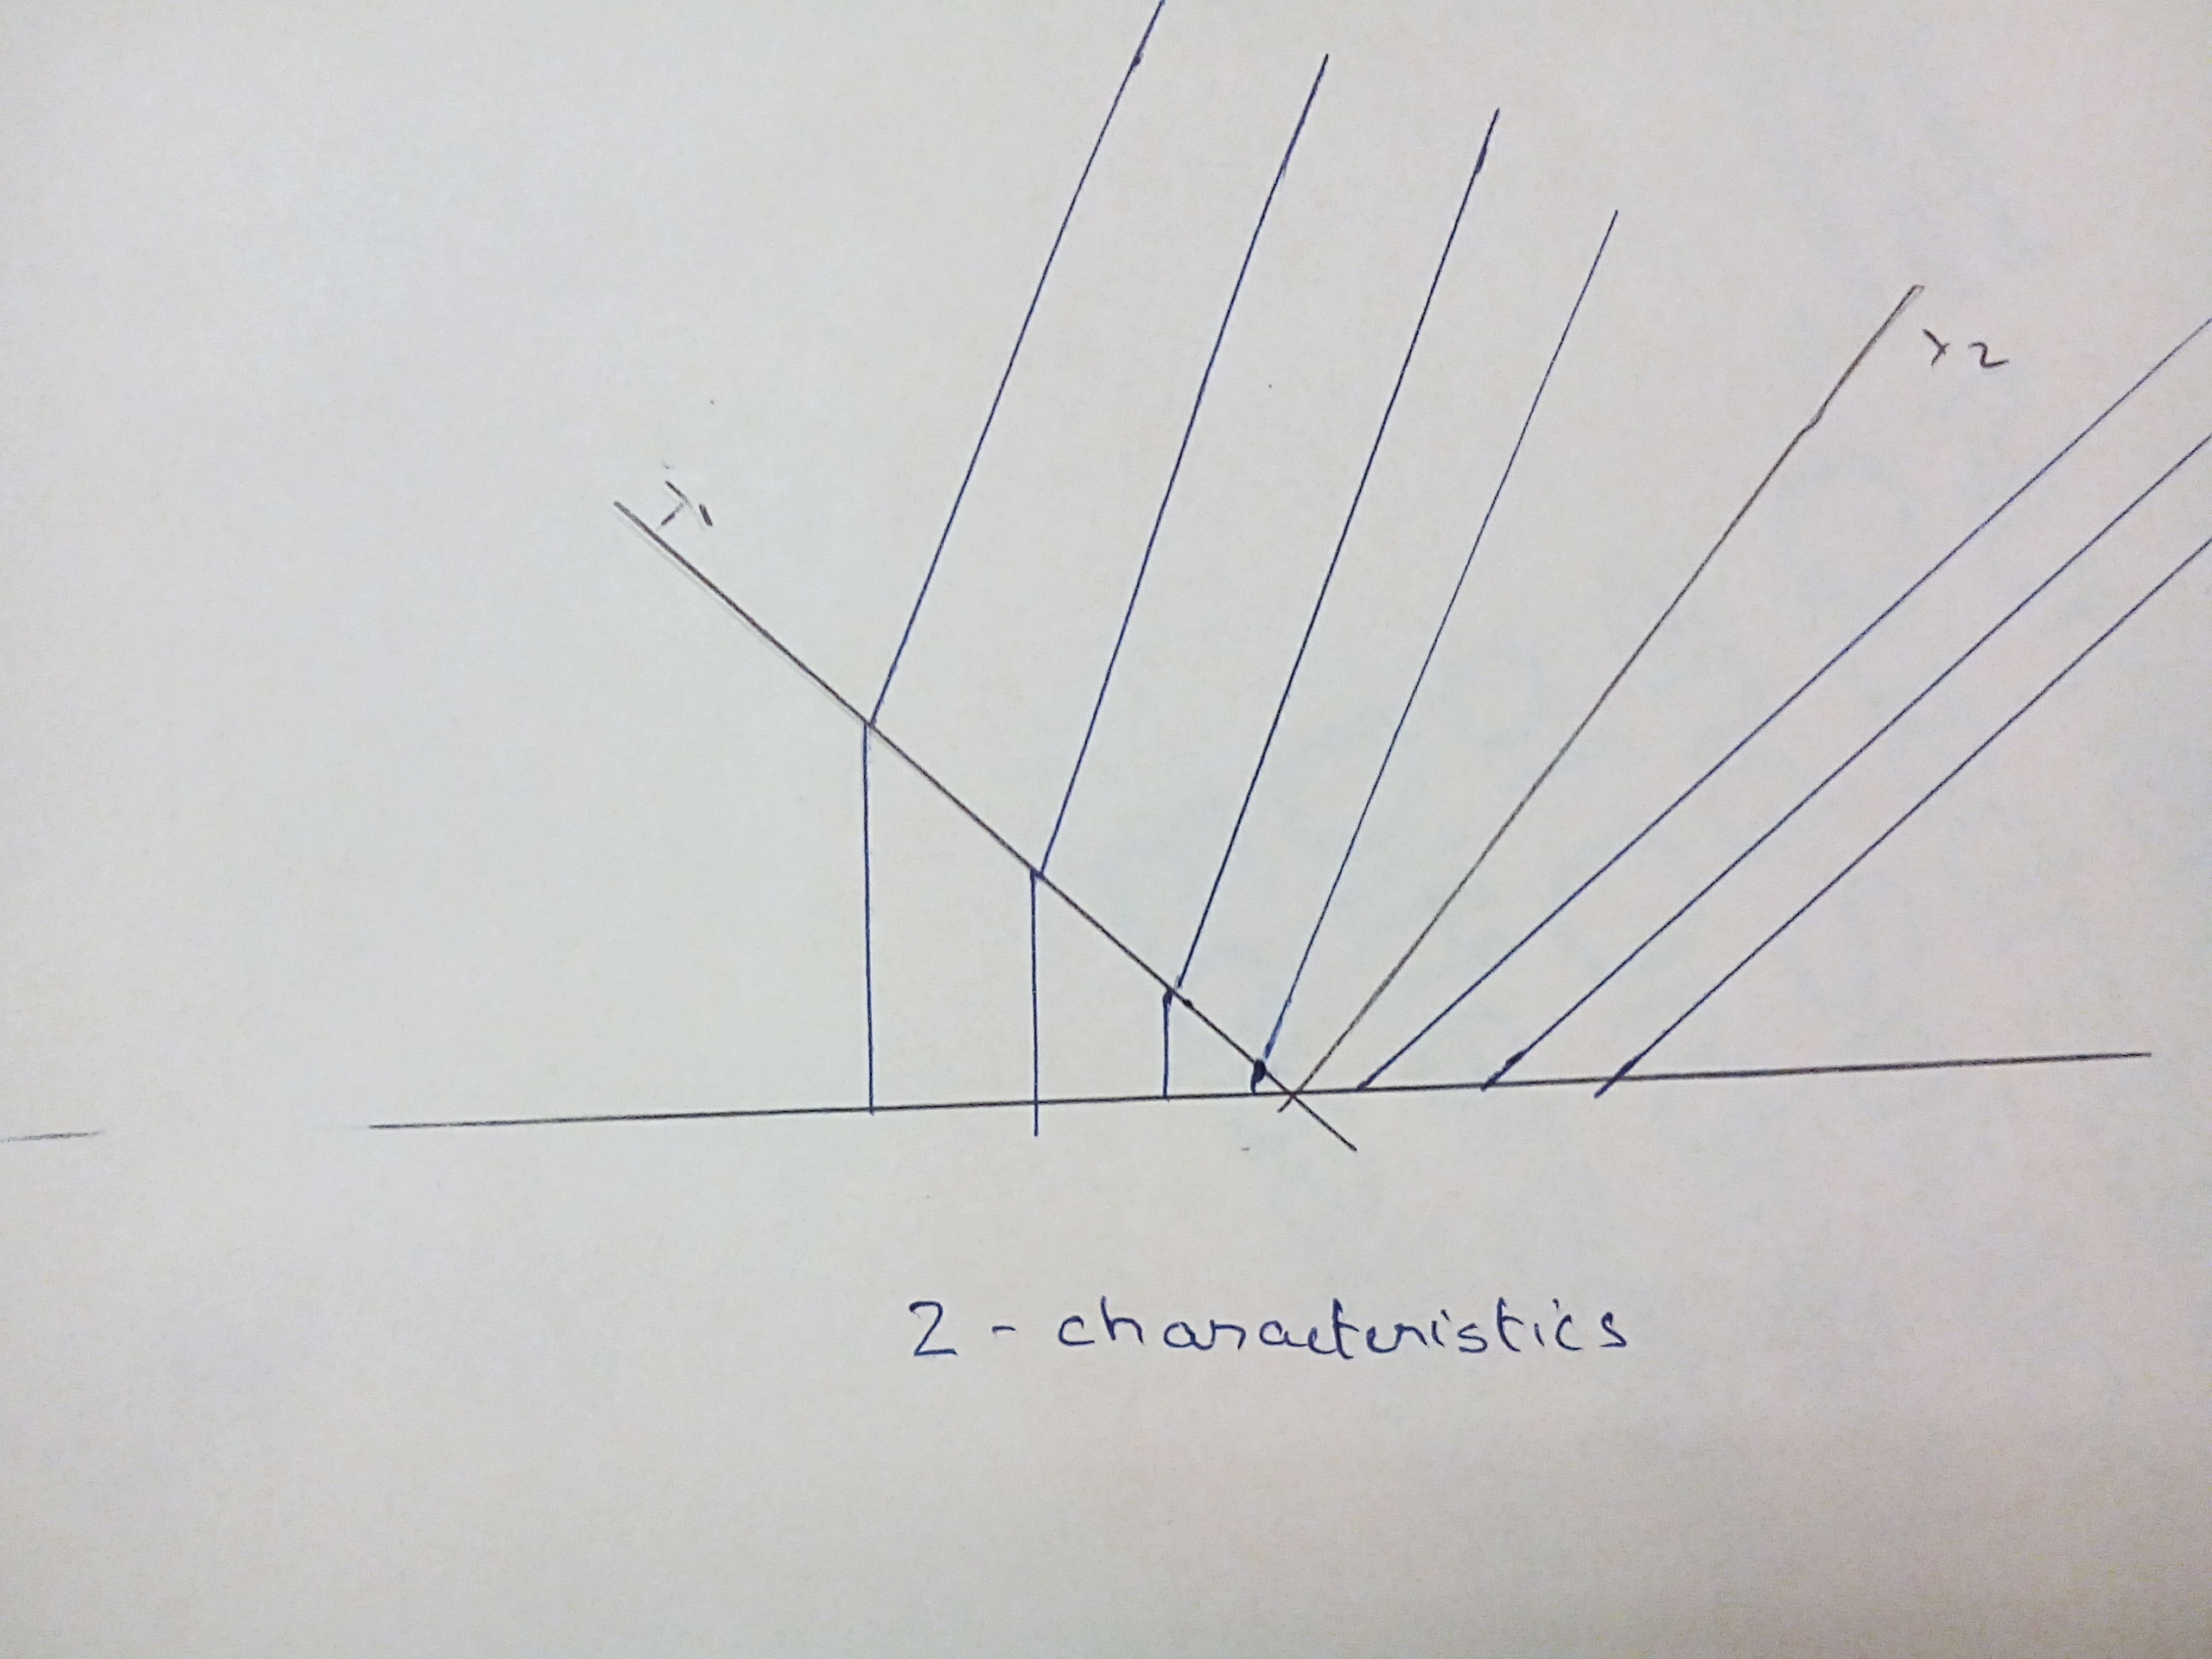
\includegraphics[width=8cm]{im2}
  \end{minipage}

\vskip 1cm
\item For the given left state $q_\ell = (1,1)$, in what region of the phase 
plane must the
right state $q_r$ lie in order for the 2-shock Riemann solution to satisfy
the Lax Entropy Condition?  
(This is already done in the notebook, you'll have to do something similar
in 2(f) below.) 

\vskip 1cm
{\bf Solution:}
To satisfy the Lax Entropy condition, 
 \[ \lambda^1_l>\lambda^1_m\]
 \[ \lambda^2_m<\lambda^2_r\]
 
 For this to happen, 
 
\[ v_m > max(v_l, v_r)\]

Given $q_l$ = (1,1), $q_r$ has to lie such that the intersection of the 2-wave through $q_r$ with the 1-wave through $q_l$ lies to the right of both $q_r$ and $q_l$. The region is shaded in the figure below.
 
\begin{minipage}{\linewidth}
	\centering
	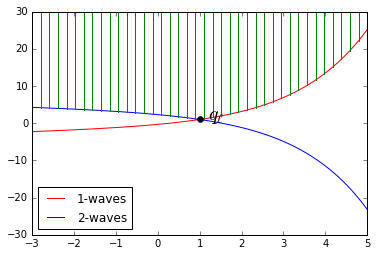
\includegraphics[width=8cm]{g.png}
\end{minipage}

\end{enumerate} 

% uncomment the next two lines if you want to insert solution...

% Or you might want to just put your solution in the Jupyter notebook!



% insert your solution here!

%--------------------------------------------------------------------------
\vskip 1cm
\hrule
\item

Consider the p-system of Problem 1 with $p(v) = -e^v$.

\begin{enumerate}
\item Follow the procedure of 13.8.1 to show that along any
integral curve of $r^1$ the relation 
\[
u = u_* - 2\left( e^{v_*/2} - e^{v/2}\right)
\]
must hold, where $(v_*,u_*)$ is a particular point on the integral curve.
Conclude that 
\[
w^1(q) = u - 2e^{v/2}
\]
is a 1-Riemann invariant for this system.

\vskip 1cm
{\bf Solution:}
 Along any integral curve of $r^1$,
 \[q' = \alpha r^1\]
 \[r^1 = \bcm 1\\  \sqrt{-p'(v)}\ecm= \bcm 1\\  e^{v/2}\ecm \]
 Taking alpha =1,
 \[v'(\xi)= 1\]
 \[v= \xi\]
 \[u'(\xi)=e^{\xi/2}\]
  \[u(\xi)=2e^{\xi/2}+c\]
  
 Since $u(v_*)=u_*$,
  \[u(v)=u_*(v_*)+ 2e^{v/2}-2e^{v_*/2} \]
  
    \[u(v)- 2e^{v/2}=u_*(v_*)-2e^{v_*/2} \]
 
Thus,
\[
w^1(q) = u - 2e^{v/2}
\]
is the 1-Riemann invariant for this system
\item Follow the procedure of Section 13.8.5 to show that through a centered
rarefaction wave 
\[
\tilde u(\xi) = A - 2\xi,
\]
where 
\[
A = u_l - 2 e^{v_l/2} = u_r - 2e^{v_r/2},
\]
and determine the form of $\tilde v(\xi)$.

\vskip 1cm
{\bf Solution:}
\[\lambda_1=- \sqrt{-p'(v)}\]
 \[r^1 = \bcm 1\\  \sqrt{-p'(v)}\ecm= \bcm 1\\  e^{v/2}\ecm\]
\[\nabla \lambda_1 = \bcm \frac{d}{dv} (- \sqrt{-p'(v)})\\0 \ecm  = \bcm \frac{d}{dv} (- e^{v/2})\\0 \ecm = \bcm  -\frac{1}{2} e^{v/2}\\0 \ecm\] 
\[ q' = \frac{r^1}{\nabla \lambda_1 .r^1}= \bcm  -2 e^{-v/2}\\-2 \ecm\]
\[ u' = -2 \]
\[ u = -2 \xi +A \]
\[A= u + 2\xi = u_l - 2 \sqrt{- p'(v_l)} =u_r - 2 \sqrt{- p'(v_r)} \]
Thus,
\[A= u + 2\xi = u_l - 2 e^{{v_l}}/2 =u_r - 2 e^{{v_r}}/2 \]

\[ v' =-2 e^{-v/2} \]
\[ v' e^{v/2}=-2 \]
\[ 2e^{v/2}=-2\xi +2B\]
\[ e^{v/2}=-\xi +B\]
\[ v(\xi)=2 log(B-\xi) \]
where
\[ B= e^{v_l/2} -e^{v_l/2} =0  \]
\[ v(\xi)=2 log(-\xi) \]
We can get the same result by using the 1-Riemann invariant.
\item Show that this field is genuinely nonlinear for all $q$.
\vskip 1cm
{\bf Solution:}
 \[\nabla \lambda_1 . r^1 = -\frac{1}{2} e^{v/2} \]
  This is never equal to zero for all finite values of q. 
\item Determine the 2-Riemann invariants and the form of a 2-rarefaction.
\vskip 1cm
{\bf Solution:}
Along any integral curve of $r2$,
\[q' = \alpha r^2\]
\[r^2 = \bcm 1\\ - \sqrt{-p'(v)}\ecm= \bcm 1\\ - e^{v/2}\ecm \]
Taking alpha =1,
\[v'(\xi)= 1\]
\[v= \xi\]
\[u'(\xi)=-e^{\xi/2}\]
\[u(\xi)=-2e^{\xi/2}+c\]

Since $u(v_*)=u_*$,
\[u(v)=u_*(v_*)- 2e^{v/2}+2e^{v_*/2} \]

\[u(v)+ 2e^{v/2}=u_*(v_*)+2e^{v_*/2} \]

Thus,
\[
w^2(q) = u + 2e^{v/2}
\]
is the 2-Riemann invariant for this system

For the 2-rarefaction,
\[\lambda_2= \sqrt{-p'(v)}\]
\[r^2 = \bcm 1\\  -\sqrt{-p'(v)}\ecm= \bcm 1\\  -e^{v/2}\ecm\]
\[\nabla \lambda_2 = \bcm \frac{d}{dv} ( \sqrt{-p'(v)})\\0 \ecm  = \bcm \frac{d}{dv} ( e^{v/2})\\0 \ecm = \bcm  \frac{1}{2} e^{v/2}\\0 \ecm\] 
\[ q' = \frac{r^2}{\nabla \lambda_2 .r^2}= \bcm  2 e^{-v/2}\\-2 \ecm\]
\[ u' = -2 \]
\[ u = -2 \xi +A \]
\[A= u + 2\xi = u_l - 2 \sqrt{- p'(v_l)} =u_r - 2 \sqrt{- p'(v_r)} \]
Thus,
\[A= u + 2\xi = u_l - 2 e^{{v_l}}/2 =u_r - 2 e^{{v_r}}/2 \]

\[ v' =2 e^{-v/2} \]
\[ v' e^{v/2}=-2 \]
\[ 2e^{v/2}=2\xi +2B\]
\[ e^{v/2}=\xi +B\]
\[ v(\xi)=2 log(B+\xi) \]
where
\[ B= e^{v_l/2} -e^{v_l/2} =0  \]
\[ v(\xi)=2 log(\xi) \]

\item Suppose arbitrary states $q_\ell$ and $q_r$ are specified and we wish to
construct a Riemann solution consisting of two ``rarefaction waves'' (which
might not be physically realizable).   Determine the point $q_m =
(v_m,u_m)$ where the two relevant integral curves intersect.
\vskip 1cm
{\bf Solution:}
\[u_m(v)=u_l(v_l)+ 2e^{v_m/2}-2e^{v_l/2} \]
\[u_m(v)=u_r(v_r)- 2e^{v_m/2}+2e^{v_r/2} \]

\[4e^{v_m/2}=u_r(v_r)-u_l(v_l)+2e^{v_r/2} +2e^{v_l/2}\]
\[v_m=2log(\frac{u_r(v_r)-u_l(v_l)+2e^{v_r/2} +2e^{v_l/2}}{4})\]

$u_m$ can be then found using the first equation.


\item What conditions must be satisfied on $q_\ell$ and $q_r$ for this to be
the physically correct solution to the Riemann problem?


In particular, for the left state $q_\ell = (1,1)$, 
shade the region of phase space where $q_r$ must lie in order to have the
Riemann solution consist of two rarefaction waves.

\vskip 1cm
{\bf Solution:}

For the solution to be valid, the terms inside the log function must be positive. So,
\[u_r(v_r)-u_l(v_l)+2e^{v_r/2} +2e^{v_l/2} \geq 0 \]



For a 2-rarefaction solution, $ \lambda^1_r >\lambda^1_m$ and $\lambda^2_m  > \lambda^2_l $. 

Since $\lambda^1 = -e^{v/2}$ and $\lambda^2 = e^{v/2}$, this means $v_m$ should lie to the left of both $v_l$ and $v_r$.

The following figure shows the possible states of $q_r$ for which the 2-wave through $q_r$ intersects the 1-wave through $q_l$ such that $v_m$ lies to the left of both of them.


\begin{minipage}{\linewidth}
	\centering
	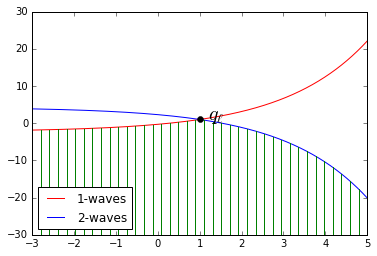
\includegraphics[width=8cm]{2g.png}
\end{minipage}

\item Determine the correct Riemann solution (consisting of one shock and
one rarefaction wave) for  the problem with
\[
q_\ell = (1,1), \qquad q_r = (4,3).
\]

\end{enumerate}

% uncomment the next two lines if you want to insert solution...
\vskip 1cm
{\bf Solution:}

This is obtained by finding the intersection of the 1-Hugoniot curve through $q_l$ and the 2-integral curve through $q_r$.

\begin{minipage}{\linewidth}
	\centering
	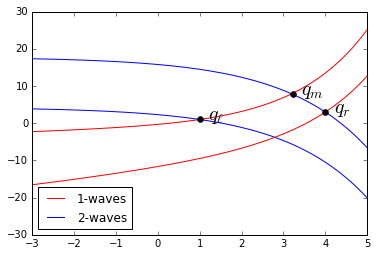
\includegraphics[width=8cm]{2f.png}
\end{minipage}

Using fsolve, we can find
\[q_m = \bcm  3.19466\\ 7.89844 \ecm\]
% insert your solution here!

%--------------------------------------------------------------------------
\vskip 1cm
\hrule
\item
For the general p-system of Problem 1,
determine the condition on the function $p(v)$
that must be satisfied in order for both fields to be genuinely nonlinear
for all $q$.

\vskip 1cm
{\bf Solution:}

 \[r^1 = \bcm 1\\  \sqrt{-p'(v)}\ecm \]
  \[r^2 = \bcm 1\\  -\sqrt{-p'(v)}\ecm \]
\[\nabla \lambda_1 = \bcm \frac{p''(v)}{2 \sqrt{- p'(v)} }\\  0\ecm  \]
\[\nabla \lambda_2 =   \bcm -\frac{p''(v)}{2 \sqrt{- p'(v)} }\\  0\ecm  \]

Thus, for genuine non-linearity ,
 \[\nabla \lambda_p . r^p \neq 0 \]
 That means
 
 \[\frac{p''(v)}{2 \sqrt{- p'(v)} }\neq 0 \]
 
 
%--------------------------------------------------------------------------
\vskip 1cm
\hrule
\item
Again consider the p-system.  For given states $q_\ell$ and $q_r$, 
define the matrix $\hat A(q_\ell,q_r)$ as
\[
\hat A = \bcm 0&-1\\ \frac{p(v_r)-p(v_\ell)}{v_r - v_\ell} & 0\ecm.
\]

\begin{enumerate} 
\item Show that this matrix satisfies the condition 
\[
\hat A (q_r - q_\ell) = f(q_r) - f(q_\ell).
\]
corresponding to equation (15.18) in the book.  This means we can
solve the linear Riemann problem $q_t + \hat A q_x = 0$ with left and right
states $q_\ell$ and $q_r$ to obtain an approximate Riemann solution that has
nice properties as described in Section 15.3.2.  Since (15.18) is satisfied,
this is called a ``Roe solver''.

\vskip 1cm
{\bf Solution:}
\[\hat A (q_r -q_l) = \bcm 0&-1\\ \frac{p(v_r)-p(v_\ell)}{v_r - v_\ell} & 0\ecm   \bcm v_r - v_l\\ u_r - u_l\ecm =   \bcm  -u_r + u_l\\ p(v_r)-p(v_\ell)\ecm = f(q_r) - f(q_\ell) \]
\item Let  
\[
c = \sqrt{\frac{p(v_r)-p(v_\ell)}{v_r - v_\ell}}
\]
Show that the eigenvalues and eigenvectors of $\hat A$ are:
\[
\Lambda = \bcm -c&0\\ 0&c\ecm, \qquad R = \bcm 1&1\\c&-c \ecm
\]
and compute the inverse $R^{-1}$.  The waves in the approximate Riemann
solution are then ${\cal W}^1 = \alpha^1 r^1$ and 
${\cal W}^2 = \alpha^2 r^2$ where $\alpha = R^{-1}(q_r - q_\ell)$.  You will
need to use this in the next problem.

\vskip 1cm
{\bf Solution:}
\[\lambda^2 = \frac{-(p(v_r)-p(v_\ell))}{v_r - v_\ell}\]
\[\lambda = \pm \sqrt{ \frac{-(p(v_r)-p(v_\ell))}{v_r - v_\ell}}\]

Thus, if 
\[c =   \sqrt{ \frac{-(p(v_r)-p(v_\ell))}{v_r - v_\ell}}\]

\[
\Lambda = \bcm -c&0\\ 0&c\ecm, \qquad R = \bcm 1&1\\c&-c \ecm
\]
 and
\[R^{-1} = \frac{1}{2} \bcm 1 & -\frac{1}{c}  \\ 1 & \frac{1}{c}\ecm\]

\end{enumerate} 

% uncomment the next two lines if you want to insert solution...
%\vskip 1cm
%{\bf Solution:}

% insert your solution here!

%--------------------------------------------------------------------------
\vskip 1cm
\hrule
\item

The sample code in \verb+$AM574/homeworks/hw4/swe_collide+ solves the
shallow water equations for a case similar to what is shown in Figure 13.19,
illustrating that when two shocks collide in a nonlinear system the
resulting interact gives waves in both families.

Using this code as a starting point, implement the Roe solver for the p-system 
in a modified version of the shallow water Riemann solver.  Note that it
will be much simpler since you don't need to worry about an entropy fix.

Clean up the code and document it so that it doesn't contain extraneous
things left over from the shallow water equations.  Create a new directory
\verb+psystem+ containing this code.

Test your code for initial data consisting of the Riemann problem with a
single jump, with 
\[
q_\ell = (1,1), \qquad q_r = (4,3)
\]
as studied above.  

Solve on the domain $-5 \leq x \leq 5$ for $0\leq t \leq 0.5$,
using 1000 grid cells.  

By examining the output files in the \verb+_output+ directory,
confirm that the intermediate
state observed in the numerical solution agrees to at least 2 or 3
significant digits with the exact intermediate state $q_m$ you found in Problem
2(g).  Note that even though an approximate Riemann solver is used in
the numerical method, it should converge to the exact solution of the
Riemann problem as the grid is refined, when viewed at some fixed time.

% uncomment the next two lines if you want to insert solution...
\vskip 1cm
{\bf Solution:}

We get the following middle state 
\[q_m = \bcm  3.1948\\ 7.897 \ecm\] which is in the order of our previous calculations.


\begin{minipage}{\linewidth}
	\centering
	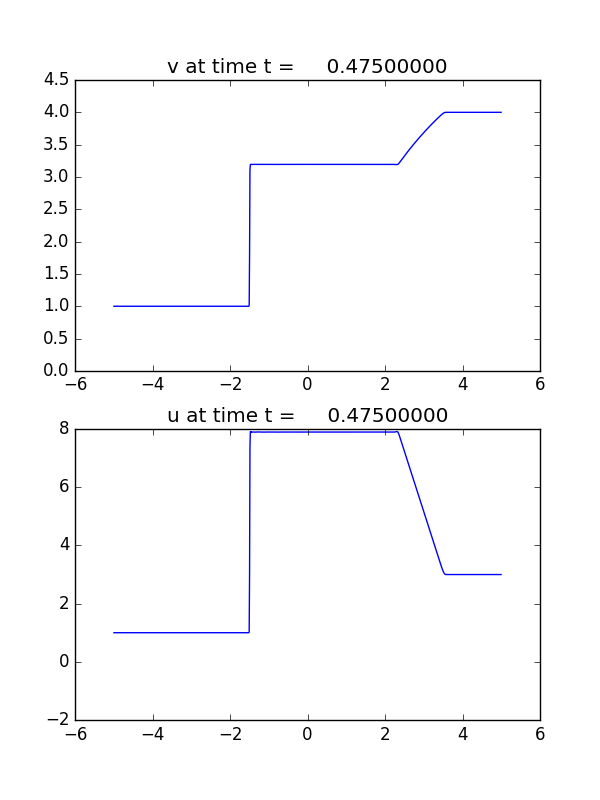
\includegraphics[width=8cm]{frame2.png}
\end{minipage}
% insert your solution here!

\end{enumerate} 

\end{document}

